\documentclass[fleqn]{report}
\usepackage{fullpage}
\usepackage{titlesec}
\usepackage{amsmath}
\usepackage{mathtools}
\usepackage{graphicx}
\usepackage{hyperref}
\graphicspath{ {./figs/} }
\DeclareUnicodeCharacter{2212}{-}
\titleformat{\chapter}[display]{\normalfont\bfseries}{}{0pt}{\Huge}
\renewcommand{\baselinestretch}{2}
\providecommand{\abs}[1]{\left\vert#1\right\vert}

\begin{document}
	\begin{titlepage}
		\begin{center}
			\textbf{\Huge K- Means Clustering\\ Uber Pickup Data NYC}{\Huge}\\
			\text{\large Project Report}\\
			\vspace{1.5cm}
			\textbf{\Large Devananth V}\\
			\text{EP20BTECH11004}\\
			\textbf{\Large Nikhil Krishna A R}\\
			\text{ME20BTECH11031}\\
			\vspace{1.5cm}
			\textbf{\LARGE Data Science and Analysis\\ Course Code:EP4130}\\		
			\vspace{1cm}	
			\begin{figure}[!h]
				\centering
				
\includegraphics[scale=0.1]{/iith.png}	
			\end{figure}	
			\vspace{1cm}
			\text{\Large Supervisor: Shantanu Desai}\\
			\text{\large May 2023}\\
		\end{center}
	\end{titlepage}
	\tableofcontents
	\begin{abstract}
		In this project we analyse the Uber pickup data NYC of april 2014. We apply k means clustering on the dataset and divide the area into clusters. We also analyse the time vs Uber pickup frequency in weekdays and weekends.\\
		The dataset used in this analysis is the Uber Pickups in New York City dataset from Kaggle, which contains information on the frequency of Uber pickups in New York City over a period of six months. We use only the month of data of April 2014 for our project.\\
		In this report, we will explore how K-means clustering can be used to analyze the frequency of Uber pickups in different areas.
	\end{abstract}
	\chapter{Introduction}
	\section{Clustering}
	Cluster analysis aims at grouping data objects based only on information found in the data that de-
	scribes the objects and their relationships. The objective of clustering is to produce groupings of things that are similar to (or connected to) one another and distinct from (or unrelated to) one another. The better, or more distinct the clustering, the greater the homogeneity  inside a group and the greater the difference across groups. Cluster analysis has always been crucial in a wide range of fields, including statistics, biology, pattern recognition, information retrieval, machine learning, and data mining, it is sometimes only a starting point for other objectives like data summarization, whether for understanding or utility.\\
	There are various kinds of clustering methods depending on the need and application at hand. In this
	work, we present one of the oldest and most used clustering technique - The K-means. 
	
	\section{K-means Clustering}
	K-Means Clustering is an Unsupervised Learning algorithm, which groups the unlabeled data set into
	different clusters. Based on a similarity measure such as euclidean distance between points, it tries to
	make the inter-cluster data points as similar as possible while also keeping the clusters as different(far)
	as possible. It assigns data points to a cluster such that the sum of the squared distance between the
	data points and the cluster’s centroid (arithmetic mean of all the data points that belong to that cluster)
	is at the minimum. The less variation we have within clusters, the more homogeneous (similar) the data
	points are within the same cluster.
	

	\subsection{K-Means Algorithm}
	Given a set of $n$ observations $\{\mathbf{x}_1, \mathbf{x}_2, \dots, \mathbf{x}_n\}$ and a desired number of clusters $k$, the K-means clustering algorithm proceeds as follows:
	\begin{enumerate}
	\item Initialize $k$ cluster centers $\{\mathbf{c}_1, \mathbf{c}_2, \dots, \mathbf{c}_k\}$ randomly or using a predefined method.
	\item Repeat until convergence:
	\begin{itemize}
	\item Assign each observation $\mathbf{x}_i$ to the cluster with the closest center $\mathbf{c}_j$ based on the Euclidean distance $d(\mathbf{x}_i, \mathbf{c}_j) = \sqrt{\sum_{p=1}^d (x_{ip} - c_{jp})^2}$, where $d$ is the dimensionality of the data.\\
	\item Recalculate the cluster centers $\mathbf{c}_1, \mathbf{c}_2, \dots, \mathbf{c}_k$ as the mean of the observations assigned to each cluster:
	\begin{align}
	\mathbf{c}_j = \frac{1}{n_j} \sum_{i=1}^n \mathbf{x}_i \cdot [j = \mathrm{argmin}_l d(\mathbf{x}_i, \mathbf{c}_l)],
	\end{align}
	where $n_j$ is the number of observations assigned to cluster $j$.	
	\item The algorithm terminates when the cluster assignments no longer change or a maximum number of iterations is reached.	
	\item The objective function of K-means clustering is the sum of squared distances between each observation and its closest cluster center:
	\begin{align}
	J = \sum_{i=1}^n \min_{j=1}^k d(\mathbf{x}_i, \mathbf{c}_j)^2.
	\end{align}	
	The algorithm aims to minimize this objective function by finding optimal cluster centers that minimize the inertia.
	\end{itemize}
	\end{enumerate}
	\chapter{Analyzing the Dataset}
	In this project we will analyse the dataset : Uber trip data from 2014 (April)\\
	There are six files of raw data on Uber pickups in New York City from April to September 2014. We only consider the data for April, 2024. The file has has the following columns:
	\begin{enumerate}
		\item Date/Time : The date and time of the Uber pickup
		\item Lat : The latitude of the Uber pickup
		\item Lon : The longitude of the Uber pickup
		\item Base : The TLC base company code affiliated with the Uber pickup
	\end{enumerate}
	\section{Plotting the Data}
	\subsection{Ride Volume by Date}
	First we will make a bar plot of uber rides per day in April 2014.
	\begin{figure}[!ht]
		\centering
		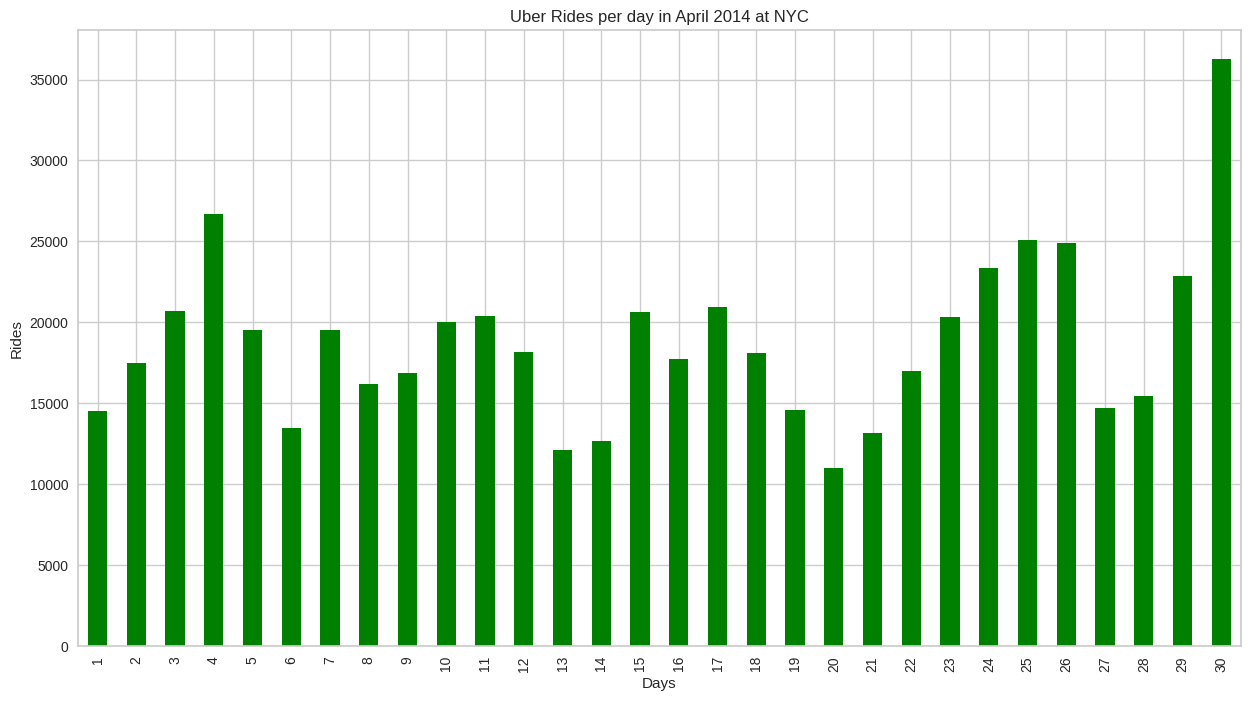
\includegraphics[scale=0.4]{/date.png}
		\caption{Total Rides Vs Date}
		\label{fig:date}
	\end{figure}\\\\
	From the plot, it seems that the daily ride volumes follow a cyclical pattern.
	\subsection{Ride Volume by Days in Week}
	Based on the previous plot, it seems like there might also be a pattern throughout the weeks.\\
	To confirm this, we can create another plot based on the days of the week.
	\begin{figure}[!ht]
		\centering
		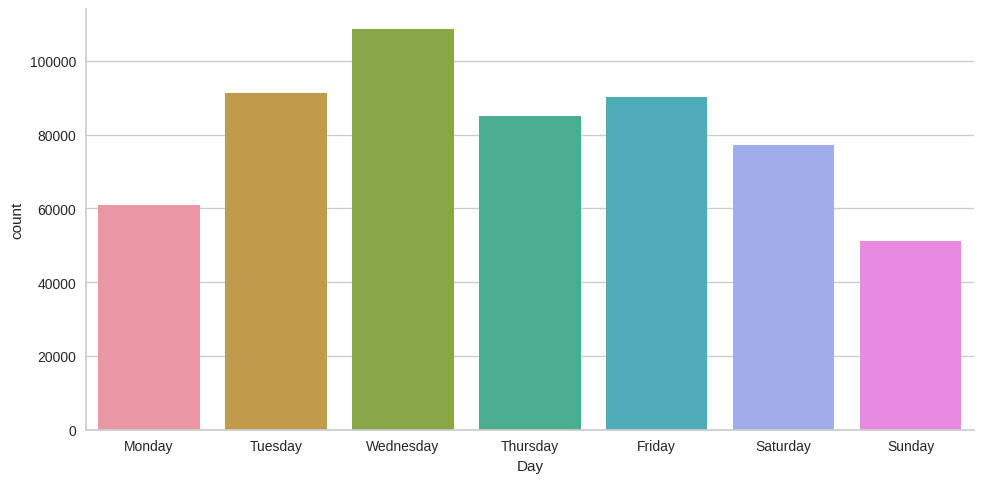
\includegraphics[scale=0.4]{/day.png}
		\caption{Total Rides Vs Day}
		\label{fig:day}
	\end{figure}\\
	\subsection{Ride Volume by Hours}
	We can also plot the ride occurrences by hours of a day.
	\begin{figure}[!ht]
		\centering
		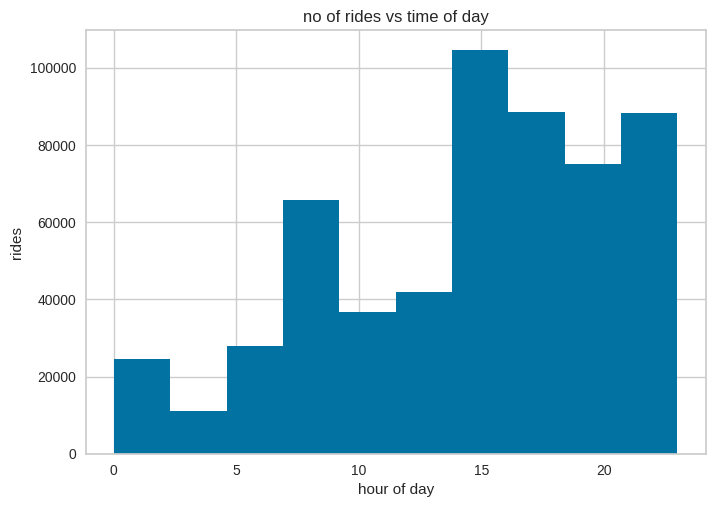
\includegraphics[scale=0.4]{/hour.png}
		\caption{Total Rides Vs Hours}
		\label{fig:hours}
	\end{figure}\\
	\subsection{Observation}
	It appears that Monday and Sunday have the least counts, while Tuesday and Wednesday have the most rides.\\
	The plot indicates that approximately 60$\%$ of rides occurred between 14:00 - 21:00.\\
	Possible Reason:
	\begin{itemize}
		\item Commuting patterns: Tuesdays and Wednesdays are typically busy weekdays when people commute to work and go about their regular activities. This could explain the higher ride counts on these days. In contrast, Mondays and Sundays may see fewer rides as people may be off work or have more flexible schedules.
		\item Business travel: Tuesdays and Wednesdays are often popular days for business travel, as professionals may travel to different locations for meetings, conferences, or other work-related events. This could contribute to the higher ride counts on these days compared to Mondays and Sundays.
		\item Weekend leisure activities: Mondays and Sundays may see fewer rides as people may prefer to stay at home or engage in leisure activities closer to their residences during weekends, resulting in lower ride counts.
	\end{itemize}
	\section{Clustering the Data}
	\subsection{Elbow Method}
	We use the elbow method to find the number of ideal clusters(k) to be used.
	\begin{figure}[!ht]
		\centering
		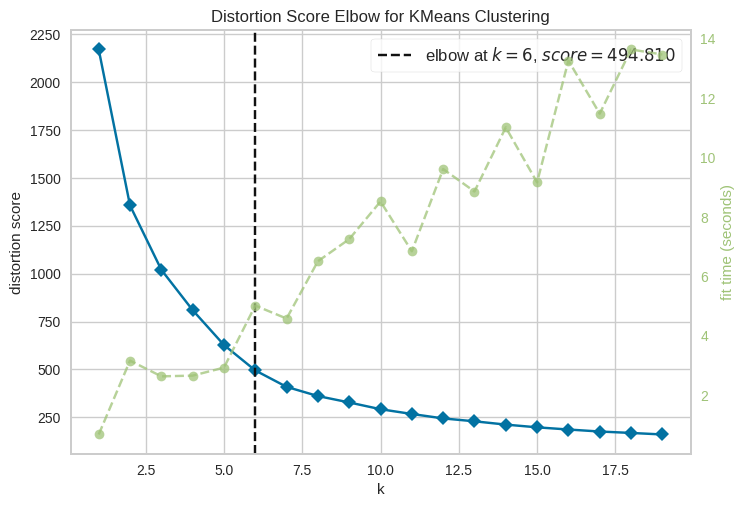
\includegraphics[scale=0.6]{/elbow.png}
		\caption{Elbow Method}
		\label{fig:elbow}
	\end{figure}
	\subsection{Finding the Centroids}
	We find the K-Means clustering to find k number of clusters and their respective centroids.\\
	We plot the centroid using Lattitude and Longitude.
	\begin{figure}[!ht]
		\centering
		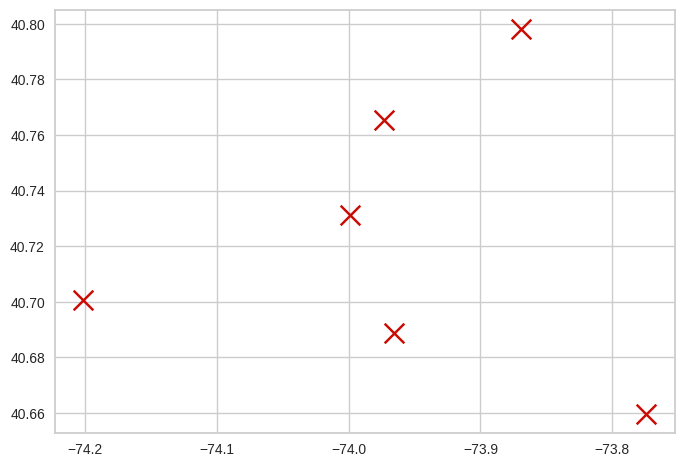
\includegraphics[scale=0.6]{/centroid.png}
		\caption{Elbow Method}
		\label{fig:centroid}
	\end{figure}\\
	Now, we use the "folium" package available in python to plot the centroids on a map.
	\begin{figure}[!ht]
		\centering
		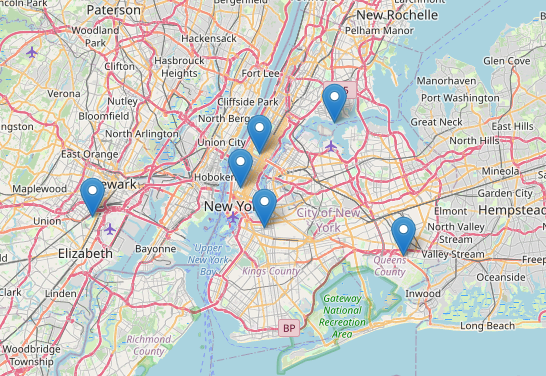
\includegraphics[scale=0.5]{/map.png}
		\caption{Hotspots}
		\label{fig:map}
	\end{figure}\\ 
	The Map shows the areas with the most probability of getting a pickup. It is helpful for a uber driver to wait in this area, so as to get the more number of pickup request. Also the the pickup point on an average will be shortest from them.
	
	\section{Clusters}
	The image given below gives the scatter plot of the clusters we got by K-means method.
	 \begin{figure}[!ht]
	 	\centering
	 	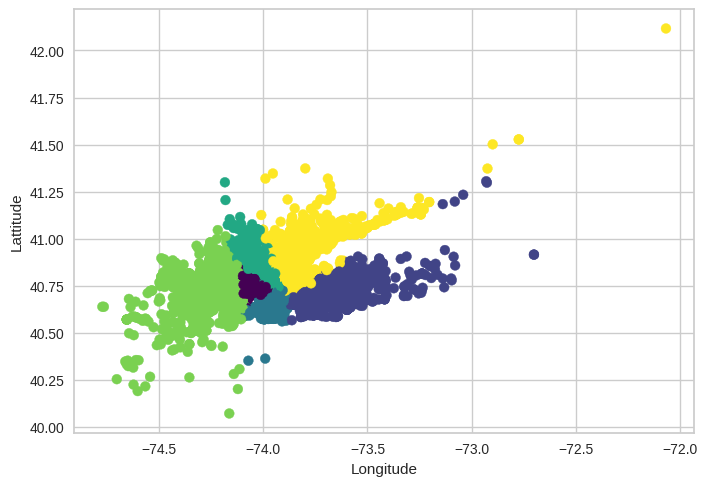
\includegraphics[scale=0.5]{/scatter.png}
	 	\caption{Clusters}
	 	\label{fig:scatter}
	 \end{figure}\\ 
 	The plot given below shows the number of pickups vs cluster.
 	\begin{figure}[!ht]
 		\centering
 		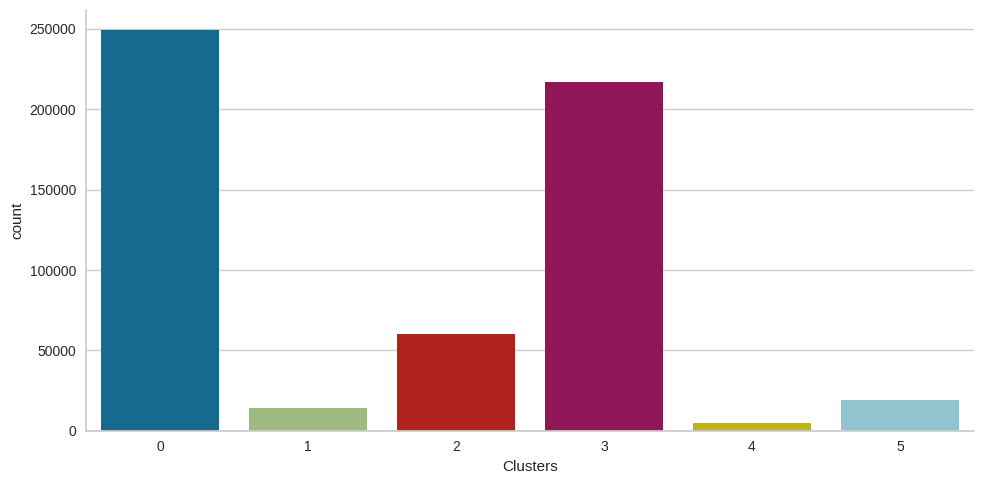
\includegraphics[scale=0.3]{/clust.png}
 		\caption{No of Pickups per Cluster}
 		\label{fig:clust}
 	\end{figure} 
 	The plots given below shows number of rides per day vs time for each of the cluster.
 	 \begin{figure}[!ht]
 		\centering
 		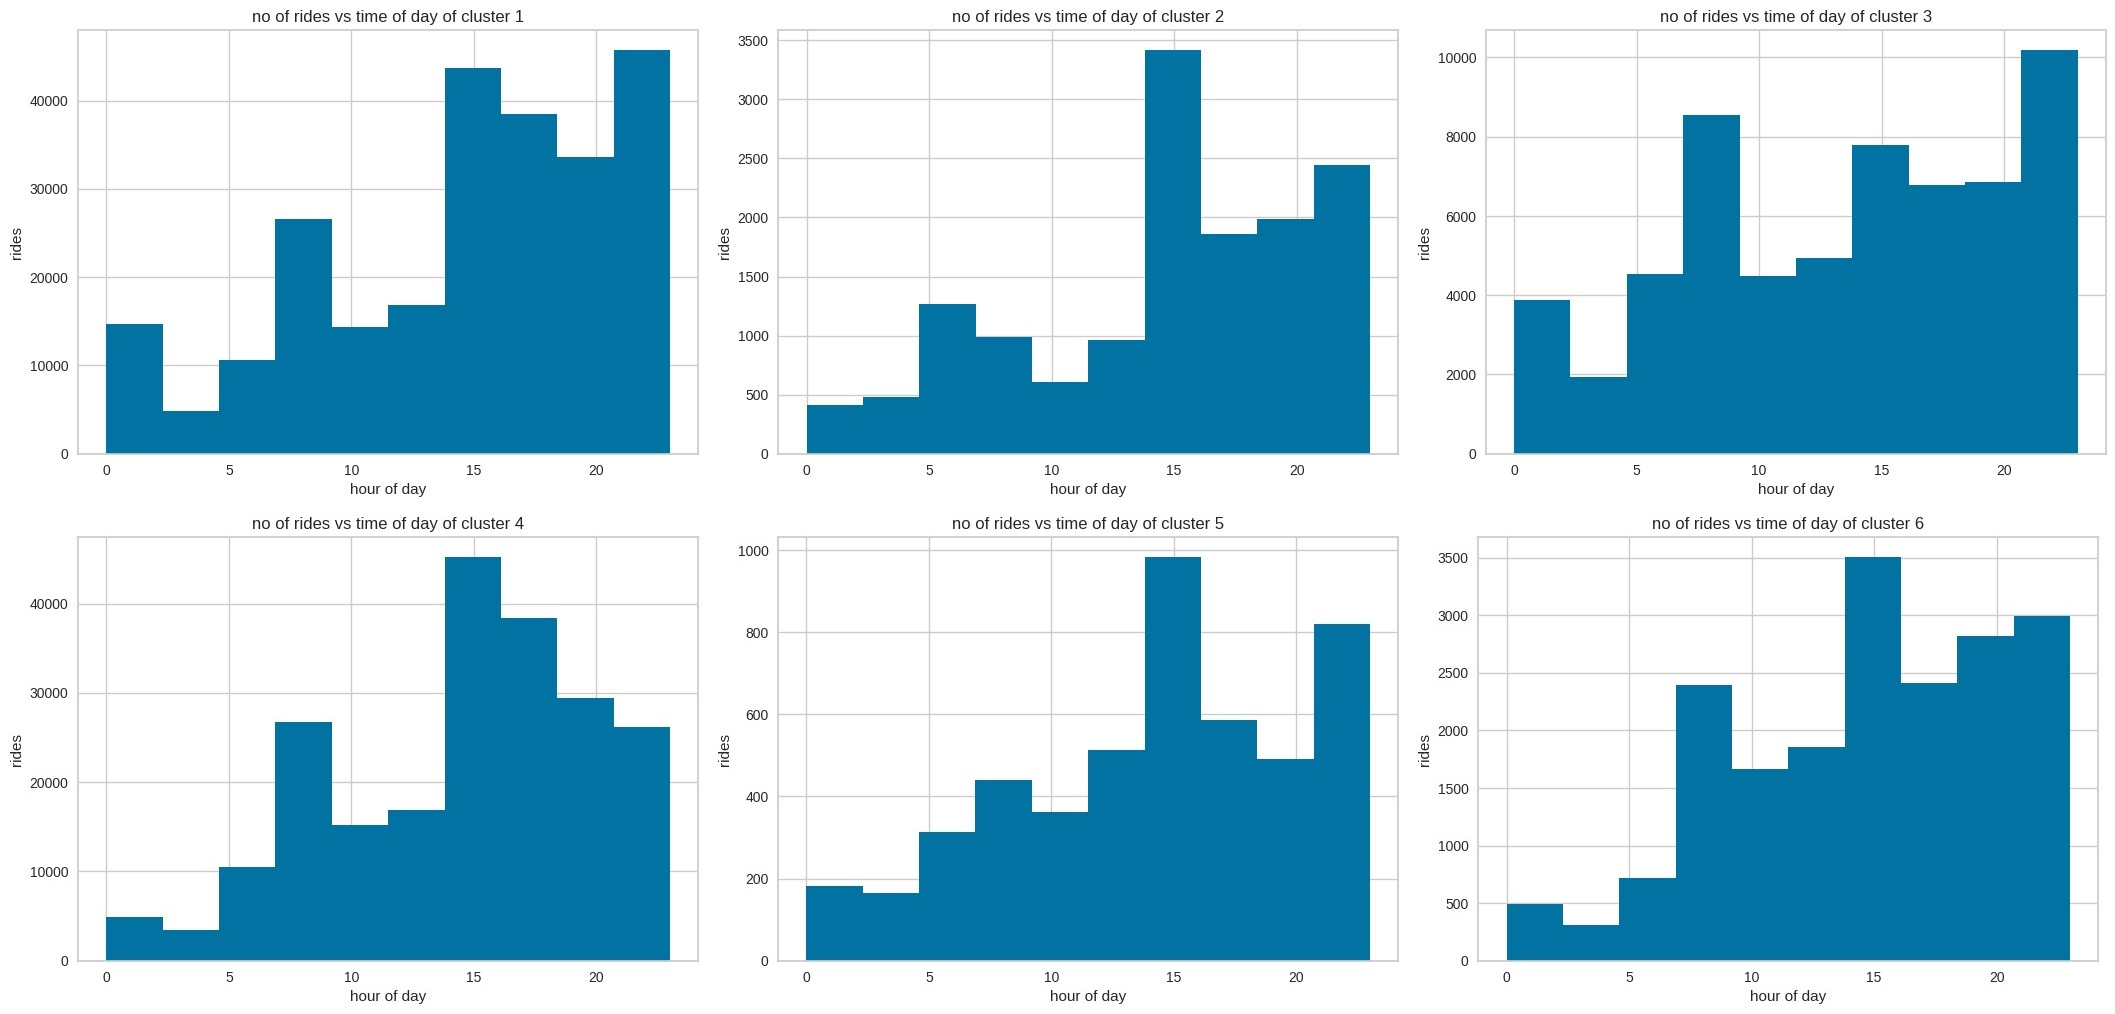
\includegraphics[scale=0.165]{/clusttime.png}
 		\caption{No of Rides Vs Time per Cluster}
 		\label{fig:c}
 	\end{figure} 
  	\section{Weekdays and Weekends}
  	Now we compare the data for weekdays and weekends.\\
  	\subsection{Weekdays}
  	The plot shows number of pickups Vs day.
  	 \begin{figure}[!ht]
  		\centering
  		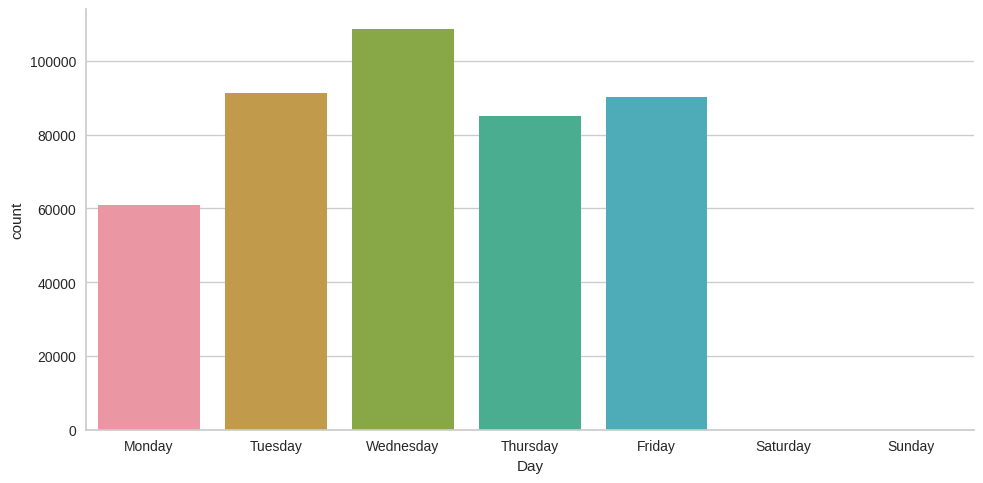
\includegraphics[scale=0.4]{/wday.png}
  		\caption{No of Pickups Vs Day}
  		\label{fig:wday}
  	\end{figure} 
  	Then we find the hotspots for this data.
  	  	 \begin{figure}[!ht]
  		\centering
  		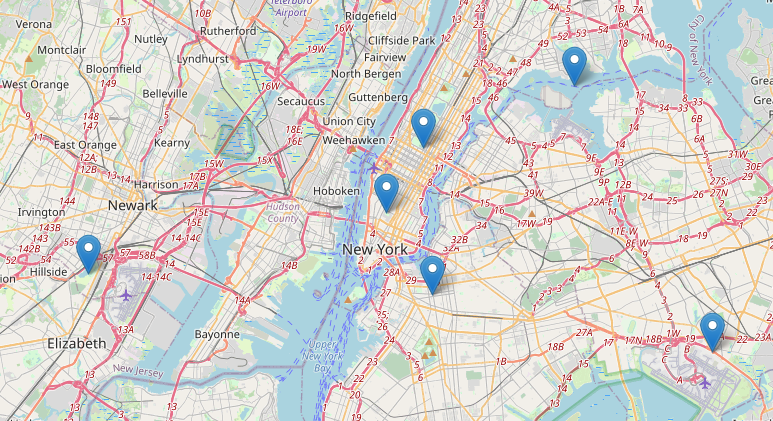
\includegraphics[scale=0.4]{/wdaymap.png}
  		\caption{No of Pickups Vs Day}
  		\label{fig:wdaymap}
  	\end{figure}\\ 
  	  	\subsection{Weekends}
  	The plot shows number of pickups Vs day.
  	\begin{figure}[!ht]
  		\centering
  		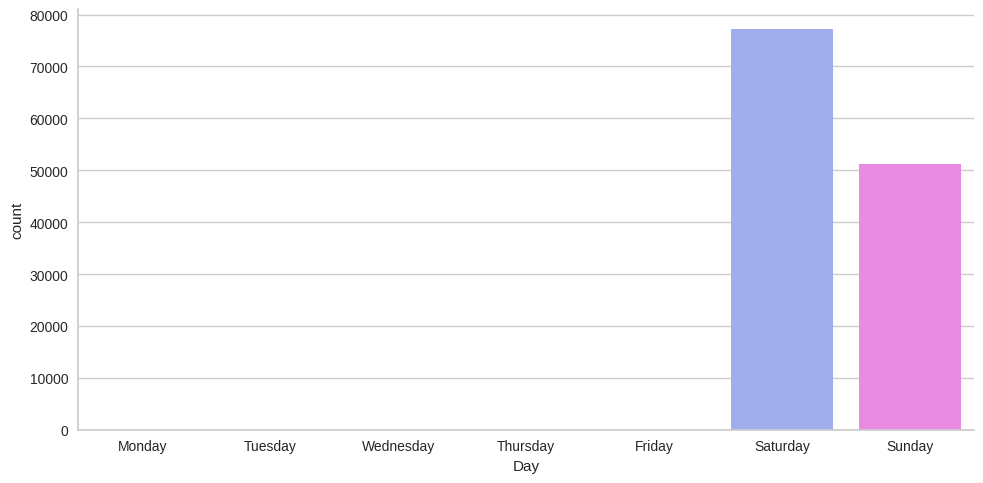
\includegraphics[scale=0.4]{/wedays.png}
  		\caption{No of Pickups Vs Day}
  		\label{fig:weday}
  	\end{figure} 
  	Then we find the hotspots for this data.
  	\begin{figure}[!ht]
  		\centering
  		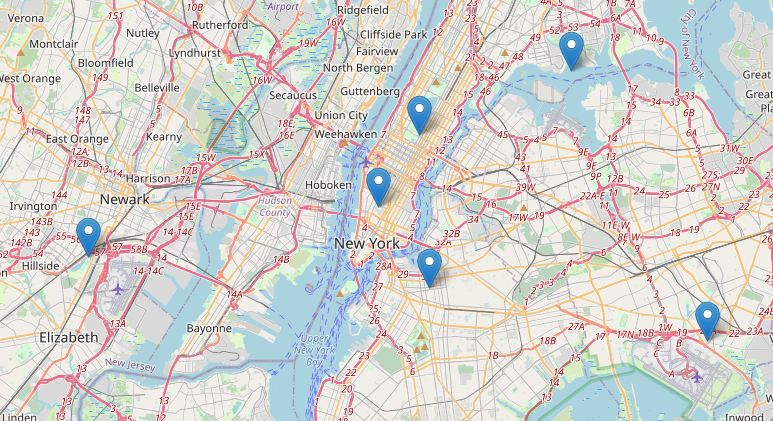
\includegraphics[scale=0.4]{/wedaymap.png}
  		\caption{No of Pickups Vs Day}
  		\label{fig:wedaymap}
  	\end{figure} \\
	\section{Acknowledgement}
	We would like to thank Prof. Shantanu Desai for giving us this wonderful opportunity to credit the
	project work we have done and for teaching the concepts in class.
	\section{Code Repository}
	\url{https://github.com/Devan2120/Data_Science/Uber_Pickup-NYC}
	\section{References}
	\begin{itemize}
		\item K-means Clustering : Wikipedia 
	\end{itemize}
	 

	
\end{document}